 \documentclass[11pt]{amsart}

\usepackage[nocompress]{cite} % puts in-text citation numbers in order

\usepackage[normalem]{ulem}
%\usepackage{subfloat}
\usepackage{subfigure}
\usepackage{caption}
%\usepackage{subcaption}
\usepackage{amsaddr}
\usepackage{color}
%\usepackage{enumitem}
\usepackage{enumerate}
%\usepackage{natbib}
\usepackage{bbm}
\usepackage[mathscr]{eucal}
\usepackage{verbatim}
\usepackage{hyperref}
\usepackage{graphicx}
\usepackage{mathtools}
\usepackage[margin=1in]{geometry}
\usepackage{amsmath}
\usepackage{amssymb}
\newcommand*{\QEDB}{\hfill\ensuremath{\square}}%

\newcommand{\foot}[1]{\mbox{}\marginpar{\raggedleft\hspace{0pt}\tiny #1}}
%\newcommand{\foot}[1]{}
\newcommand{\NN}{\mathbb{N}}
\newcommand{\ZZ}{\mathbb{Z}}
\newcommand{\sign}{{\rm sign}}
\newtheorem{definition}{Definition}[section]
\newtheorem{notation}{Notation}[section]
\newtheorem{theorem}{Theorem}[section]
\newtheorem{lemma}[theorem]{Lemma}
\newtheorem{proposition}[theorem]{Proposition}
\newtheorem{corollary}[theorem]{Corollary}
\newtheorem{thma}{Theorem}
\renewcommand{\thethma}{\Alph{thma}}
\theoremstyle{remark}
\newtheorem*{remark}{Remark}


\numberwithin{equation}{section}
\newcommand{\reals}{\mathbb{R}}
\newcommand{\ones}{\mathbf{1}}
\DeclareMathOperator*{\argmin}{arg\,min}

%\usepackage{authblk}
%\usepackage{caption}
%\usepackage{subcaption}

\def\presuper#1#2%
  {\mathop{}%
   \mathopen{\vphantom{#2}}^{#1}%
   \kern-\scriptspace%
   #2}

\DeclareMathOperator*{\IGP}{\presuper{IGP}{\mathit{A}}}
\DeclareMathOperator*{\Tri}{\presuper{Tri}{\mathit{A}}}
\DeclareMathOperator*{\MRS}{{\rm MRS}}
\DeclareMathOperator*{\SSS}{{\rm SS}}
%\DeclareMathOperator*{\NS}{NS}
\newcommand{\NS}{NS}

\newcommand{\mn}{\color{blue}}

\newcommand{\themethod}{containment min hash }
\DeclareMathOperator{\Jac}{{\rm Jac}}


% % % % % % % % % % % % % % % %
% Potential reviewers:
% 

% % % % % % % % % % % % % % % % % % % % % % % % % % % % % % % % % % % % % %

\begin{document}



\title[Improving Min Hash]{Improving Min Hash for Metagenomic Taxonomic Profiling} %Inside the square brackets is the running head


\author{Hooman Zabeti${}^{1}$, David Koslicki${}^{1*}$}
\address{${}^1$ Mathematics Department, Oregon State University, Corvallis, OR.}
\thanks{${}^*$ Corresponding Author: \url{david.koslicki@math.oregonstate.edu}}





\date{\today}
\begin{abstract}
Abstract here.  \\\\
\smallskip
\noindent \textsc{Keywords}: \emph{Min hash, k-mins sketch, metagenomics, taxonomic profiling, taxonomic classification, Jaccard index, containment}.
\end{abstract}
\maketitle


\section{Introduction}
\begin{enumerate}
\item Min hash recently has been used to great success on biological data
\item Mash, Titus' sourmash
\item originally designed for sets of relatively similar size and appreciable intersection size
\item metagenomic taxonomic profiling the setup is different: many relatively small database entries, one very large metagenomic sample, very small intersection sizes in general
\item we modify the min hash paradigm to this particular situation so it can handle a sample of much greater size than the reference database entries.
\end{enumerate}

Min hash is great at comparing sets of similar size. When one set is much larger than the other, the Jaccard index is going to be smaller, which by the Chernoff bounds is where it has a hard time. In metagenomics, the typical paradigm is one very large set (the metagenomic sample) call it $B$ and a bunch of small reference/database sets (call one $A$). Taking the classical min hash approach means sampling from $A\cup B$. Part a) of Figure \ref{fig:Conceptual} demonstrates such a situation while sampling 100 random points of $A\cup B$ and leads to \input{Data/ClassicalConceptual.txt}points lying in $A\cap B$. On the other hand, if we sample from just $A$ (instead of $A\cup B$) and have some way to test if a point $x$ is in $A\cap B$, we would get a much better estimate of $|A\cap B|$. Part b) of Figure \ref{fig:Conceptual} demonstrates this approach while sampling only 50 points from $A$ and finds \input{Data/ContainmentConceptual.txt}points lying in $A\cap B$. They key to our approach is that the membership test $x\in A\cap B$ can be efficiently performed with a bloom filter of $B$. We analyze the time and space complexity, as well as the accuracy of this approach and find that for parameters typically used in metagenomics, our proposed approach is faster, uses less space, and is more accurate than the classical min hash approach.


\begin{figure}[!h]%
\begin{center}
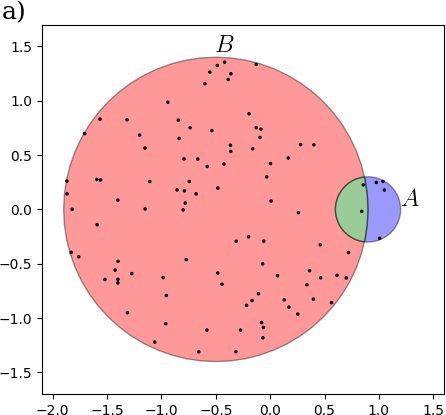
\includegraphics[width=3.15in,trim={0 0 0 0in},clip]{Figs/ClassicalConceptual.png}%
\hspace{1ex}
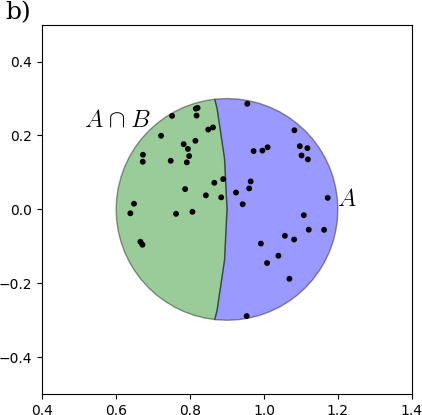
\includegraphics[width=3.0in,trim={0 0 0 0in},clip]{Figs/ContainmentConceptual.png}
\end{center}
\caption{Conceptual comparison of classical min hash to the proposed containment approach when estimating the Jaccard index of very different sized sets. a) Sampling 100 points from $A\cup B$ (as is done in the classical min hash approach) leads to finding only \protect \input{Data/ClassicalConceptual.txt}elements in $A\cap B$. b) Sampling just 50 points of $A$ and testing if a point $x\in A\cap B$, finds \protect \input{Data/ContainmentConceptual.txt}elements in $A\cap B$. This latter approach will be seen to lead to a better estimate of the Jaccard index. }
\label{fig:Conceptual}%
\end{figure}





\section{Methods}
Definitions, derivation of mathematical results here.
\subsection{Definitions}
\begin{enumerate}
\item Definitions of database entries, query sample, k-mer size, note size disparity
\item define classic min hash (k-independent version and k-mins version)
\item define the containment approach
\end{enumerate}
\subsection{Min Hash via containment}
\label{section:ChernoffBounds}
\subsection{Time and space complexity}
\begin{enumerate}
\item Chernoff bound estimates
\item comparison of number of hashes required for same accuracy
\item time complexity
\item space complexity (all with examples of the numbers in practice).
\end{enumerate}


\section{Results}
In this section, we compare classic min hash to the proposed method.
\subsection{Synthetic data}
\label{section:SyntheticData}
Here we illustrate the improved accuracy of \themethod over classical min hash in estimating the Jaccard index. To that end, we generated two random strings $w_A$ and $w_B$ on the alphabet $\{A,C,T,G\}$. We set $|w_A|= 10,000$ and $|w_B| = 15$ to simulate the situation of interest where one wishes to estimate the Jaccard index of two sets of very different size. We then appended a common string $w_C$ of increasing length to each of $w_A$ and $w_B$ so that $\Jac_k(w_Aw_C, w_Bw_C)$ ranges between 0 and 1. We picked the $k$-mer size of $11$ and utilized a signature size of 100. Figure \ref{fig:TrueVsEstimate} depicts the comparison of \themethod with the classical min hash Jaccard estimate on this data and effectively illustrates the results in section \ref{section:ChernoffBounds} which proved that the containment approach has a higher probably of being closer to the true Jaccard than the classic approach. The mean and variance of the classic min hash approach on this data was \input{Data/SyntheticDataClassic.txt}while using the containment approach was \input{Data/SyntheticDataContainment.txt}demonstrating a substantial decrease in variance. This improved variance was observed over a range of $k$-mer sizes, number of hashes, and lengths of input strings.


\begin{figure}[!h]%
\begin{center}
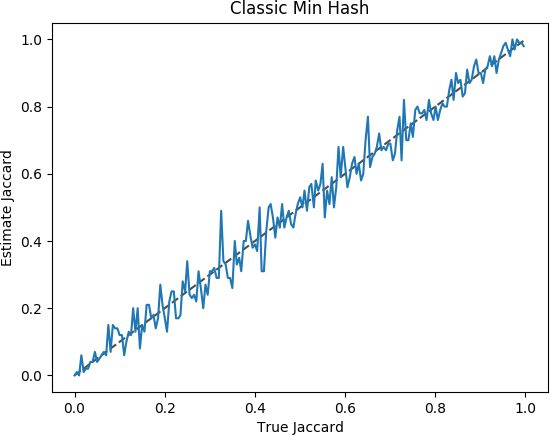
\includegraphics[width=3.25in,trim={0 0 0 0in},clip]{Figs/TrueVsEstimate.png}%
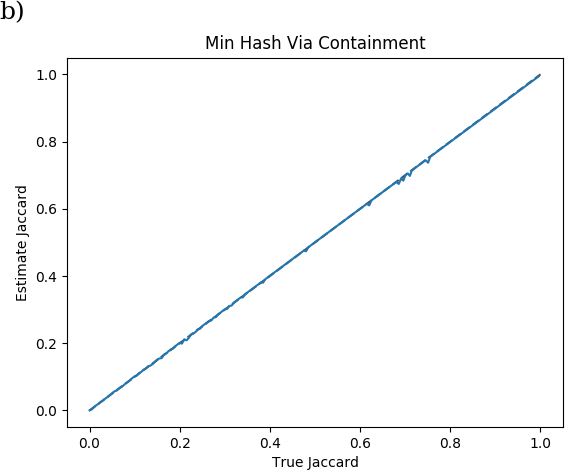
\includegraphics[width=3.25in,trim={0 0 0 0in},clip]{Figs/ContainmentTrueVsEstimate.png}
\end{center}
\caption{Comparison of \themethod to the classical min hash estimate of the Jaccard index on synthetic data. Each method utilized the 100 smallest hashes of the murmer3 hash function on the $11$-mers of two randomly generated strings with sizes 10,000 and 15 respectively after appending a common substring of increasing size. a) Classical min hash estimate of the Jaccard index. b) The proposed \themethod method on the same data.}
\label{fig:TrueVsEstimate}%
\end{figure}


\subsection{Simulated biological data}
To demonstrate the exponential improvement of \themethod over classical min hash for increasing sample sizes, we contrast here the mean relative performance of the classical min hash estimate to the containment approach on simulated biological data. We utilized GemSIM \cite{mcelroy2012gemsim} to simulate two sets of metagenomic data. The first set had an average number of $k$-mers in the sample was only \input{Data/SimulatedBiologicalData_small_rel_size.txt}of the size of the average number of $k$-mers in the genomes used to simulate the data. The second set had an average number of $k$-mers in the sample equal to \input{Data/SimulatedBiologicalData_rel_size.txt}of the average size of the number of $k$-mers in the genomes used to simulate the data. As demonstrated in Section \ref{section:ChernoffBounds} we expect that once the number of $k$-mers in the sample is large in comparison to the number of $k$-mers used to simulate the data, the containment approach will give an exponentially better estimate of the Jaccard index in comparison to the classical min hash approach. Figure \ref{fig:SimulatedBiologicalData} depicts the relative error of the classic min hash approach and the containment approach on these two sets of simulated data. Observe that the containment approach has significantly less error when, as is commonly seen in practice, the number of $k$-mers in the sample is appreciable in comparison to the number of $k$-mers in a given reference organism. As demonstrated in section \ref{section:ChernoffBounds}, this improvement of the containment approach over the classic approach continues to grow as the metagenome size grows in relation to the reference genome sizes.

For the first set of simulated data, we used GemSIM to simulate \input{Data/SimulatedBiologicalData_small_NumReads.txt}reads from \input{Data/SimulatedBiologicalData_small_NumGenomes.txt}randomly selected bacterial genomes for the $k$-mer size $k=\input{Data/SimulatedBiologicalData_small_ksize.txt}$. We then repeated this \input{Data/SimulatedBiologicalData_small_NumReplicates.txt}times. A false positive rate of \input{Data/SimulatedBiologicalData_small_p.txt}was used for the false positive rate of the bloom filter used for the containment approach.

For the second set of simulated data, we used GemSIM to simulate \input{Data/SimulatedBiologicalDataNumReads.txt}reads from \input{Data/SimulatedBiologicalDataNumGenomes.txt}randomly selected bacterial genomes for the $k$-mer size $k=\input{Data/SimulatedBiologicalDataksize.txt}$. We then repeated this \input{Data/SimulatedBiologicalDataNumReplicates.txt}times. A false positive rate of \input{Data/SimulatedBiologicalDatap.txt}was used for the false positive rate of the containment approach.

\begin{figure}[!h]%
\begin{center}
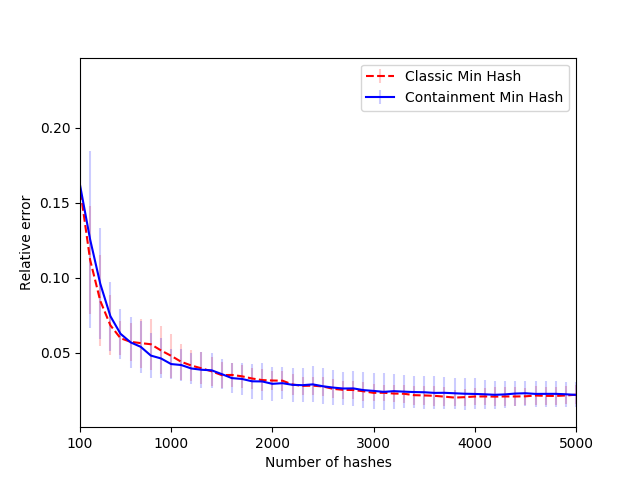
\includegraphics[width=3.25in,trim={0 0 0 0in},clip]{Figs/SimulatedBiologicalData_small.png}%
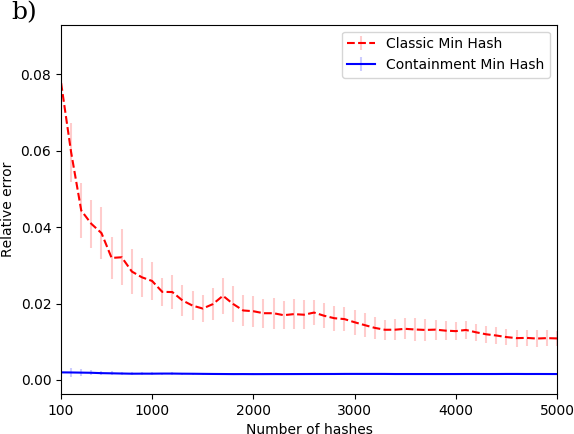
\includegraphics[width=3.25in,trim={0 0 0 0in},clip]{Figs/SimulatedBiologicalData.png}
\end{center}
\caption{Comparison of relative error of \themethod to the classical min hash estimate of the Jaccard index on simulated biological data. a) On \protect \input{Data/SimulatedBiologicalData_small_NumReplicates.txt}replicates of samples consisting of \protect \input{Data/SimulatedBiologicalData_small_NumGenomes.txt}genomes with only  \protect \input{Data/SimulatedBiologicalData_small_NumReads.txt}reads. b) On \protect \input{Data/SimulatedBiologicalDataNumReplicates.txt}replicates of samples consisting of \protect \input{Data/SimulatedBiologicalDataNumGenomes.txt}genomes with \protect \input{Data/SimulatedBiologicalDataNumReads.txt}reads.
}
\label{fig:SimulatedBiologicalData}%
\end{figure}

\subsection{Real biological data}

Real metagenomes contain many magnitudes more $k$-mers than those found in any reference organisms \cite{} which indicates the advantage of utilizing the proposed containment approach to the classical min hash estimate of the Jaccard index. To evaluate the utility of the containment min hash approach on real biological data, we analyzed a subset of DNA generated by the study in \cite{howe2014tackling} consisting of those reads contained in the sample 4539585.3.fastq. This sample consisted of 25.4M reads with average length of 65bp. We formed a bloom filter consisting of all 21-mers of this sample and formed sketches of size 500 from 4,798 viral genomes obtained from NCBI. Utilizing the proposed containment min hash approach, we found the largest containment index between the reference viral metagenomes and the sample to be \input{Data/FoundOrganismContainment.txt}for the virus \textit{\input{Data/FoundOrganismName.txt}}which corresponds to a Jaccard index of \input{Data/FoundOrganismJaccard.txt}\unskip. As demonstrated in section \ref{section:ChernoffBounds} we can be XX\% sure that the true Jaccard index between this genome and the sample is within a relative error of XX\% of the true Jaccard index value.  If we were to use the classical min hash approach, the Chernoff bounds dictate that we would min hash sketches of size XXX to achieve this same confidence bound on the relative error.

To evaluate if this extremely low-abundance organism is actually present in the sample, we utilized the SNAP alignment tool \cite{zaharia2011faster} to align the sample to the \textit{\input{Data/FoundOrganismName.txt}}genome. The script \textit{MakeCoveragePlot.sh} provides the exact commands and parameters used to perform the alignment. We found that \input{Data/NumReadsAligned.txt}reads aligned with a MAPQ score above 10. The coverage of the viral genome is depicted in Figure \ref{fig:ViralCoverage} using a square-root scale and a window size of \protect \input{Data/WindowSize.txt}\unskip. Even though the coverage was quite low (average per-window coverage was \input{Data/MeanCoverage.txt}\unskip X), the coverage was quite uniform and consistent which lends evidence to support the claim of the presence of this particular virus in the sample metagenome.

\begin{figure}[!h]%
\begin{center}
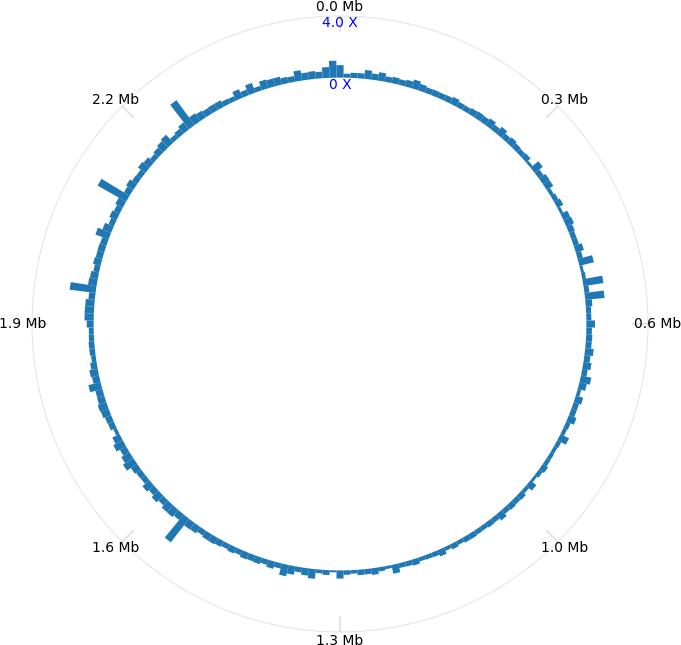
\includegraphics[width=3.25in,trim={0 0 0 0in},clip]{Figs/CoveragePlot.png}%
\end{center}
\caption{Plot of the real metagenomic sample alignment coverage to the virus \protect \textit{\protect \input{Data/FoundOrganismName.txt}} detected by the proposed containment min hash approach. A total of \protect \input{Data/NumReadsAligned.txt}reads aligned with a MAPQ score above 10 using the SNAP aligner \cite{zaharia2011faster}. A square root scale and a window size of \protect \input{Data/WindowSize.txt}was used for the plot, resulting in an average per-window coverage of \protect \input{Data/MeanCoverage.txt}\unskip X.
}
\label{fig:ViralCoverage}%
\end{figure}

\section{Discussion}


\clearpage
\bibliography{library}{}
\bibliographystyle{abbrv}

\end{document}

